\chapter{Exigences et besoins}

\section{Diagramme de cas d'utilisation}

Les diagrammes de cas d'utilisation illustrent les principales fonctionnalités de SecuCom selon les différents types d'utilisateurs du système.

Le premier diagramme présente les fonctionnalités accessibles à l'administrateur du système, qui peut gérer les utilisateurs, les rôles et permissions, ainsi que les paramètres système. Ces fonctionnalités sont essentielles pour maintenir la sécurité et la configuration globale de la plateforme.

\begin{figure}[h]
\centering
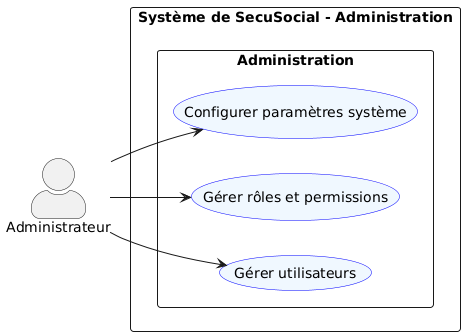
\includegraphics[width=0.8\textwidth]{AdminUC.png}
\caption{Diagramme de cas d'utilisation - Administrateur}
\end{figure}

Le deuxième diagramme illustre les fonctionnalités accessibles aux contacts des entreprises clientes. Ils peuvent gérer les informations de leur entreprise, leurs travailleurs, créer et suivre des demandes DIMONA, gérer des documents et consulter les informations relatives à la paie et à la facturation.

\begin{figure}[h]
\centering
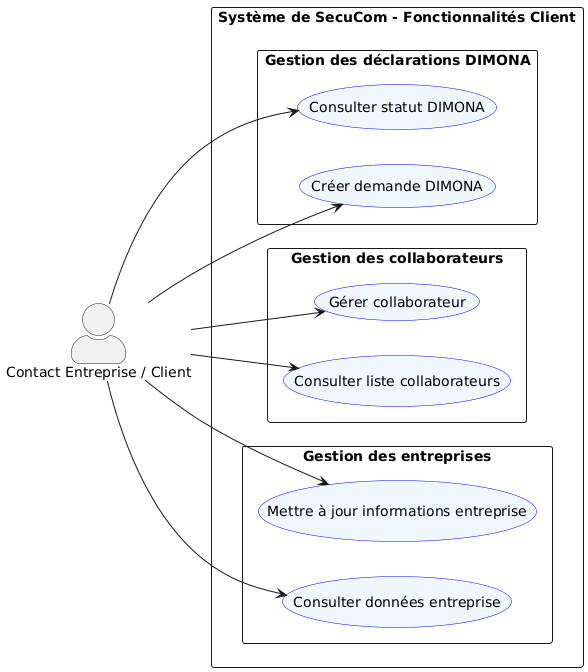
\includegraphics[width=0.8\textwidth]{ClientUC.png}
\caption{Diagramme de cas d'utilisation - Client}
\end{figure}

Le troisième diagramme présente les fonctionnalités accessibles aux employés du secrétariat social. Ils disposent d'un accès étendu pour gérer les entreprises clientes, leurs travailleurs, traiter les demandes DIMONA, gérer les documents et les prestations, ainsi que les aspects liés à la paie et à la facturation. Le système intervient également pour certaines actions automatisées comme la réception des confirmations DIMONA et les notifications.

\begin{figure}[h]
\centering
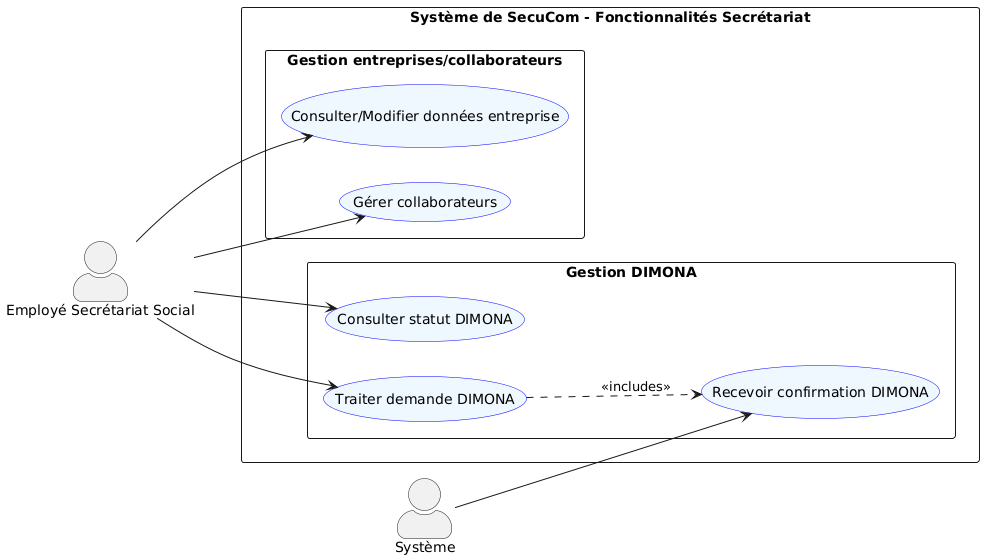
\includegraphics[width=0.8\textwidth]{SecretariatUC.png}
\caption{Diagramme de cas d'utilisation - Secrétariat Social}
\end{figure}

\section{Exigences et besoins techniques, de sécurité et de performance}

\subsection{Besoins techniques}

L'architecture technique de SecuCom a été conçue pour répondre aux exigences spécifiques d'un secrétariat social tout en garantissant évolutivité, maintenabilité et robustesse. Les choix technologiques suivants ont été retenus :

\textbf{Architecture globale} :
\begin{itemize}
  \item Architecture client-serveur avec séparation claire entre frontend et backend
  \item API RESTful pour la communication entre les différentes couches
  \item Déploiement sur serveur dédié ou cloud selon les besoins
\end{itemize}

\textbf{Frontend} :
\begin{itemize}
  \item Framework ReactJS avec TypeScript pour une meilleure maintenabilité et détection d'erreurs
  \item Interface responsive pour différentes tailles d'écran desktop (pas d'optimisation mobile)
  \item État global géré via Redux ou Context API
\end{itemize}

\textbf{Backend} :
\begin{itemize}
  \item Framework Spring Boot pour le développement d'applications Java
  \item Spring Security pour la gestion de l'authentification et des autorisations
  \item Spring Data JPA pour l'accès aux données et la persistance
  \item Hibernate comme ORM (Object-Relational Mapping)
  \item Base de données relationnelle pour le stockage des données structurées
\end{itemize}

\textbf{Modèle de données} :
Basé sur l'implémentation actuelle, le modèle de données comprend les entités suivantes :
\begin{itemize}
  \item User : utilisateur du système avec authentification
  \item SocialSecretariat : entité représentant le secrétariat social
  \item SecretariatEmployee : employé du secrétariat social
  \item Company : entreprise cliente
  \item CompanyContact : contact au sein de l'entreprise cliente
  \item Collaborator : travailleur/employé d'une entreprise cliente
  \item Dimona : déclaration DIMONA associée à un collaborateur
  \item Address : adresse physique (utilisée par plusieurs entités)
\end{itemize}

\textbf{Environnement de développement} :
\begin{itemize}
  \item Gestion de version avec Git
  \item Build automatisé avec Maven
\end{itemize}

\subsection{Besoins de sécurité}

La sécurité est un aspect fondamental de SecuCom, étant donné la nature sensible des données traitées. Les exigences de sécurité suivantes ont été implémentées :

\textbf{Authentification et autorisation} :
\begin{itemize}
  \item Authentification sécurisée basée sur JWT (JSON Web Tokens) comme implémenté dans JwtAuthenticationFilter et JwtUtils
  \item Gestion des rôles et permissions via Spring Security
  \item Séparation stricte des espaces de données entre les différentes entreprises clientes
  \item Validation des permissions à chaque requête API
\end{itemize}

\textbf{Protection des données} :
\begin{itemize}
  \item Transmission sécurisée via HTTPS/TLS
  \item Gestion des exceptions avec GlobalExceptionHandler pour éviter la fuite d'informations sensibles
  \item Conformité au RGPD (Règlement Général sur la Protection des Données)
\end{itemize}

\textbf{Sécurité applicative} :
\begin{itemize}
  \item Protection contre les attaques courantes (XSS, CSRF, injection SQL) via Spring Security
  \item Validation des entrées côté serveur avec les DTOs
  \item Gestion sécurisée des mots de passe (hachage avec sel)
  \item Mécanisme de rafraîchissement de token (RefreshTokenRequest)
\end{itemize}

\subsection{Besoins de performance}

Bien qu'aucune restriction spécifique n'ait été définie en termes de performance, SecuCom doit offrir une expérience utilisateur fluide et réactive pour garantir son adoption par les utilisateurs. Les exigences suivantes ont été établies :

\textbf{Temps de réponse} :
\begin{itemize}
  \item Chargement initial de l'application < 3 secondes
  \item Temps de réponse des requêtes API < 1 seconde pour les opérations courantes
  \item Affichage des listes et tableaux optimisé
\end{itemize}

\textbf{Capacité et évolutivité} :
\begin{itemize}
  \item Support simultané d'un nombre suffisant d'utilisateurs pour les besoins de Sodabel
  \item Capacité à gérer la croissance du nombre d'entreprises clientes et de collaborateurs
  \item Architecture permettant l'évolutivité en cas de besoin
\end{itemize}

\textbf{Disponibilité} :
\begin{itemize}
  \item Disponibilité du service adaptée aux heures de travail du secrétariat social
  \item Temps de récupération après incident raisonnable
  \item Maintenance planifiée en dehors des heures de bureau
\end{itemize}

\textbf{Optimisation} :
\begin{itemize}
  \item Requêtes SQL optimisées pour les opérations courantes via Spring Data JPA
  \item Structure de base de données efficace avec les index appropriés
\end{itemize}

Ces exigences techniques, de sécurité et de performance constituent le cadre dans lequel SecuCom a été développé, garantissant une solution robuste, sécurisée et performante qui répond aux besoins spécifiques de Sodabel et potentiellement d'autres secrétariats sociaux de taille similaire.
